\documentclass[11pt, oneside]{article}   	% use "amsart" instead of "article" for AMSLaTeX format
\usepackage{geometry}                		% See geometry.pdf to learn the layout options. There are lots.
\geometry{letterpaper}                   		% ... or a4paper or a5paper or ... 
%\geometry{landscape}                		% Activate for for rotated page geometry
%\usepackage[parfill]{parskip}    		% Activate to begin paragraphs with an empty line rather than an indent
\usepackage{graphicx}				% Use pdf, png, jpg, or eps§ with pdflatex; use eps in DVI mode
								% TeX will automatically convert eps --> pdf in pdflatex		
\usepackage{amssymb}
\usepackage{url}

\title{TestMine: Mining test evolution for improved software test selection}
\author{Wasif Afzal}
\date{}							% Activate to display a given date or no date

\begin{document}
\maketitle
\section{Introduction and motivation}\label{sec:intro}
There is an increasing reliance on software in our daily activities. This reliance mandates that software is able to meet its users' expectations, otherwise the consequences can be undesirable. During software development a range of verification and validation (V\&V) activities are performed with the goal of developing software that meets its requirements. Software testing is one major V\&V activity which aims to find \textit{as many defects as possible, as early as possible in the development phase, under given constraints of cost and schedule}~\cite{29119}. Clearly this is a challenging task, simply because there are not enough resources to test a software exhaustively. As a result, a lot of research has been done to make software testing efficient and effective. 

Software testing is typically performed at different levels, namely unit/component, integration, system and acceptance test levels. Also testing is performed as part of a specific life cycle model; agile development being the latest model. In agile, as the software is built incrementally, testing has to be a continuous process that needs to adapt with the changing nature of requirements. Issues such as timely identification of integration and regression issues and efficient system testing becomes critical concerns in an increment. %Figure~\ref{fig:agile_incr} shows an example of how testing is an integrated part of an agile increment. 

%\begin{figure} [h]
   %\centering
   %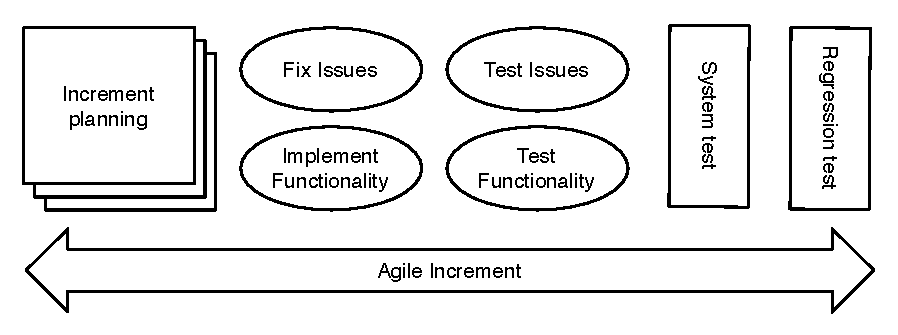
\includegraphics[width=80mm,height=35mm]{agile_incr.pdf}
   %\caption{Testing in an agile increment (adapted from~\cite{29119}).}
   %\label{fig:agile_incr}
%\end{figure}

In agile the iterations are short, e.g., in Scrum each sprint is typically lasting one and four weeks. With the addition of new functionality and continuous fixing of issues in an increment%(Figure~\ref{fig:agile_incr})
, regression testing has to be done at its best. According to Engstr\"{o}m et al.~\cite{Emelie10}, iterative development strategies require frequent retesting of previously tested functions due to changes in related code and therefore it is important to use regression strategies that are efficient. As the number of increments increase, typically the regression test suite grows in size and becomes more expensive to run in each increment. This means that re-running every test case in the test suite will be expensive. This approach is generally called as \textit{retest all} and is the simplest regression test strategy~\cite{Graves01}. It is then natural to think about regression test selection (RTS) techniques as part of the overall regression test strategy. 

RTS techniques select subset of test cases from the test suite. It differs from test suite minimization or test suite reduction problem in the sense that it is modification-aware, i.e., the selection is specific to the current version of the program and is focussed on the modified parts of the program~\cite{Yoo12}. RTS thus verifies the behaviour of modified software. More formally, given an initial program \textit{P}, an original test suite \textit{T} associated with \textit{P} and a modified version of the program \textit{P'}, RTS techniques find a subset of \textit{T}, \textit{T'} to test \textit{P'}. 

RTS techniques have its own share of challenges. Such techniques can be costly to run and can miss potentially fault revealing test cases. Therefore it is always a trade-off between time required to select and run test cases and the fault detection ability of test cases~\cite{Graves01}. This trade-off is also highlighted by Engstr\"{o}m et al.~\cite{Emelie10}: \textit{[\ldots] there is a trade-off between cost reduction and defect detection ability. This is the case in all test selections, and none of the evaluated techniques seems to have done any major breakthrough in solving this trade-off.}

There are different classification schemes for RTS techniques but the most used classification property is whether these techniques are \textit{safe} or \textit{unsafe}~\cite{Emelie10}. A safe RTS technique ensures that the test suite \textit{T'} has all tests in \textit{T} that execute code that was changed from \textit{P} to \textit{P'}~\cite{Harrold99}. So with safe RTS techniques the faults found with tests in \textit{T} are also found with tests in \textit{T'}~\cite{Emelie10}. Harrold~\cite{Harrold99} calls such tests as \textit{modification traversing} for \textit{P} and \textit{P'}.  In other words if there is a modification traversing test case in the test suite, it will definitely be selected by a safe RTS technique~\cite{Yoo12}. However Rothermel and Harrold~\cite{Rothermel96} shows that precisely identifying modification traversing tests in T is difficult in practice due to non-determinism in programs and test execution, e.g., testing of a system ported to different operating system. As a result, several RTS techniques can be found in literature with varying precision and efficiency. This, again, helps explain the trade-off that exists in RTS techniques between cost and defect detection effectiveness. An unsafe RTS technique is one that may miss tests from \textit{T'} that are modification traversing. An unsafe RTS technique may be beneficial in cases where parts of \textit{P'} remain untested (or not covered) after running \textit{T'}. A simple example of unsafe RTS technique is random selection of test cases~\cite{Emelie10}. 

Apart from the safe-unsafe classification, Yu et al.~\cite{Yu12} presents another interesting multidimensional way to classify (safe) RTS techniques in terms of \textit{software}, \textit{bug} and \textit{data} dimensions. Within the \textit{software} dimension, the two most important research directions are categorised as \textit{code-based} and \textit{model-based} approaches. In deed most of the RTS research falls in the software dimension where techniques operate at different granularity levels; Orso et al.~\cite{Orso04} differentiates between techniques operating at high-level (such as at the method or class level) and those operating at low-level (such as at the level of statements). This is to say that a large body of literature on RTS techniques analyse code, at different abstraction levels, to seek modifications in the program under test. This large body of evidence on RTS techniques focus at unit level testing. This is also acknowledged in the survey paper by Yoo and Harman~\cite{Yoo12}: \textit{``A majority of existing regression testing techniques reply upon structural information about the SUT, such as data-flow analysis, CFG analysis, program slices and structural coverage''}. The model-based approaches differ from source code being an input to having other software artefacts, such as activity diagrams and other UML based design documents. These specification-based RTS methods aim to cover certain features of the model such as all transition-pairs and all round trip paths. These methods are applicable at integration and system test levels, but as Yoo and Harman~\cite{Yoo12} points out, these model-based approaches assume the presence of traceability from specifications to code-level artefacts and test cases, which is harder to achieve in practice.  

From a \textit{bug} dimension, there are RTS methods based on the fix-cache algorithm proposed by Kim et al.~\cite{Kim07}. The test cases are linked to source code files and are prioritised depending on the fault-proneness of the files, if they are changed~\cite{Engstrom10b,Wikstrand09}. 

The third and the last dimension of RTS  techniques by Yue et al.~\cite{Yu12} is based on \textit{data} where test cases that are most likely to reveal a fault are selected (e.g., by using execution profiles as in~\cite{Zhang10}). 

What is interesting here is that the \textit{bug} and \textit{data} dimensions of RTS techniques open up opportunities to apply machine learning and data mining algorithms for RTS. This represents, in one way, a significant departure from \textit{code-based} approaches where much effort is applied to identify modifications in the program under test. Also unlike the code-based approaches for RTS, the \textit{bug} and \textit{data} dimensions of RTS techniques are more likely to be applicable to higher levels of testing, such as integration and system. Support for \textit{high-level} regression testing is also a way to extend the applicability of RTS techniques from over-simplistic, small-scale academic problems to real-world software systems as a whole. The techniques that are based \textit{only} on the data generated during software development are likely to add little overhead in terms of additional effort. It seems rational to leverage upon such techniques for reducing the cost of regression testing.

This data-centred approach of solving problems is at the heart of what we now know as \textit{software analytics}. Software analytics is about using potentially large amounts of data for real and actionable insights~\cite{Buse10}. Software analytics employs several well-known mechanisms such as trend analysis, classification algorithms, predictive analytics, optimisation, simulation and data- and text-mining.

The fundamental theme of this project is to investigate if software analytics (using test evolution data) can help select a more cost-effective and efficient test suite at system test level. Such an investigation is challenging from multiple perspectives. First, there is scarcity of research on test selection at \textit{system} test level. Given that testing at system test level occurs late in the life cycle, with potentially less time left, any intelligent selection at this level would help increase confidence in the effectiveness of system test effort. Second, many of the non-functional properties manifest best at the system level, therefore customised test suites targeting one or more of these properties can be effectively selected. Third, it is still not evident how the test selection strategies at system test level would get integrated in newer development methodologies like agile and lean. Fourth, in cases where code coverage information is missing or is deemed too expensive to gather, it is logical to make use of existing test related data to assist a selection strategy and measure how effectively the new test suite covers artefacts other than code, such as requirements. 

\section{Scientific questions}\label{sec:rq}

The purpose of this project is to use data generated during test executions (or test evolution) to help decide which test cases to select for testing at system test level. The focus here is to leverage data that is already generated and is available to be used for a selection strategy. This project will propose methods and ways to achieve cost-effective, high-level test selection. The project aims to answer the following research questions: 

\begin{enumerate}
    \item[RQ 1] How can regression test selection be done in a cost-effective manner using test evolution data?
    \item[RQ 2] What is the effectiveness and efficiency of using test evolution data for regression test selection at system test level? 
    \item[RQ 3] How can such an approach integrate effectively in agile/lean software development?
\end{enumerate} 

\section{Project's expected results and effects}\label{sec:expected_results}
It is expected that the project will result in following outcomes: 
\begin{enumerate}
  \item RTS techniques based on software test execution or software test evolution data, thus applicable in cases where detailed code coverage information might be missing or hard to gather. 
  \item RTS techniques that are applicable at higher levels of testing, e.g., at integration and system test levels.
  \item Empirical evaluation of RTS techniques on large, industrial projects to improve scalability and to promote technology transfer.
\end{enumerate}

\subsection{Project's impact on business/industrial partners}\label{sec:impact_industry}
Selection of an appropriate subset of test cases to execute so that the objectives of testing are met is expected to reduce the cost of testing. This is especially true for regression testing which remains one of the most expensive activities performed during a software system's lifecycle~\cite{Harrold99}. There is no use in running test cases with no added value, i.e., if there are no gains in terms of coverage and if the tests are not fault revealing. Removing such test cases will not only improve the test suite; it will allow more time to be spent on developing newer and more interesting (fault-revealing) test cases. Intelligent variation is essential for revealing faults in regression testing since if the same older tests are repeated for regression testing then they are incapable of finding newer faults or faults which arise due to potential side-effects of a code change. As Whittaker~\cite{Whittaker09} mentions, variation of testing focus is the key in revealing faults in regression testing. Regression test selection (RTS) techniques is one way to provide intelligent insight in the capability of a test suite.

Also, as Cartaxo et al.~\cite{Cartaxo11} notes, in practice test case selection is usually a manual and an ad hoc process that is error prone; the results of this project shall enable a systematic and an intelligent selection of test cases. This shall enable the industrial partners to have sufficient guarantees that their selection strategy is grounded in facts and real data, and is thus more effective in terms of reducing cost and finding more faults. 

%\section{Benefits for the industrial partners}\label{sec:benefit_industrial_partners}

In more concrete terms, the results of this project will benefit the industrial partners in the following ways:

\begin{enumerate}
	\item The results will improve the performance of regression testing at higher test levels (integration and system test).
	\item The improvement in the performance of regression testing at integration and system test levels would mean less cost for the development project and improved fault detection effectiveness (faults  are more costly to fix if found at the customer end).
	\item The techniques proposed in this project would help in general test selection (not necessarily in the context of regression testing) where the goal is to find a subset of the original test suite that guarantees the execution of fault revealing test cases. 
	\item The software engineers learn better and systematic ways of testing software. This includes injecting intelligent variation in the regression testing suite, thus improving test suite effectiveness and efficiency.
	\item The insight and experience gained during the implementation of this project can be extended to company-wide projects for broader benefits. 
\end{enumerate} 
	
%\subsection{}
\subsection{Project's impact on individual research and the research area}\label{sec:impact_research}
Industrial scalability and cost-effectiveness of RTS techniques at higher-levels of testing are still open research challenges, despite that there is lots of research on RTS techniques in general. There is certainly a lack of applicable methods for RTS at high-level of testing that makes use of test execution or test evolution data. Then there is evidence to suggest that RTS techniques are evaluated against a limited number of programs and test suites and hence it is desirable to engage more actively with industry to show the cost-effectiveness and usefulness of such techniques~\cite{Yoo12}. This project aims to fulfil these stated gaps in RTS research, working on which is expected to yield substantial research impact. The plan is to disseminate the expected results of this project through several conference and journal papers, thus strengthening the research profile of the applicant as well as MDH.

The goals of this project are complimentary to the expertise of the applicant and MDH. Working in co-production with [partner 1] and [partner 2] will enhance applicant's already existing knowledge in software verification and validation. This also promises to contribute positively in strengthening the newly created Software Testing Laboratory\footnote{\url{http://www.es.mdh.se/research-groups/27-Software_Testing_Laboratory}} at MDH. The applicant is part of this laboratory which has a vision of promoting industry-relevant research in software testing. The laboratory also hosts the recently awarded KKS project on Testing of Critical System Characteristics (TOCSYC)\footnote{\url{http://www.es.mdh.se/projects/349-TOCSYC___Testing_of_Critical_System_Characteristics}} in which the applicant is also a participant. [say something about spin-off or refine previous sentence more or talk to Paul on this].

\section{Project implementation}\label{sec:proj_implementation}
The planned duration of the project is 24 months. The implementation of the project is divided into several work packages (WPs) as described below. 

\subsection{WP1: Literature review and domain gathering}\label{sec:WP1}
Considering that test selection at system test level is not researched extensively, this WP shall gather what research is available on the topic. This will build a knowledge-base for the activities coming in forth-coming WPs. In parallel to the review, this WP shall start gathering domain knowledge regarding designated projects by our partner companies. This will educate the project leader about contextual variables specific to different projects under study.  \textbf{Deliverable:} The deliverable for this WP will be a conference paper for the review part.

\subsection{WP2: Data gathering and cleansing}\label{sec:WP2}
Since the target of the project is to make use of test evolution data, a fundamental step is to investigate what data is available and what is its quality. This WP will also consider if certain data pre-processing steps need to be carried out. Attribute selection and removal of redundant variables will also be considered a part of this WP.  \textbf{Deliverable:} The deliverable for this WP will be an internal artefact that will serve as an input for later WPs.

\subsection{WP3: Test selection support and solution formulation}\label{sec:WP3}
In this WP, we will devise mechanisms  for relating test evolution data for test selection. This mechanisms would include finding similarities and diversities among tests based on test evolution data. (See more from Hemmati et al. paper). It is expected that several of such mechanisms would be evaluated for both test selection effectiveness and efficiency. \textbf{Deliverable:} The deliverable for this WP will be an internal artefact that will serve as an input for later WPs.

\subsection{WP4: Experimental evaluation}\label{sec:WP4}
In this WP, the actual test selection using test evolution data from previous WPs will be carried out and the results will be evaluated for efficiency and effectiveness. Suitable measures for efficiency and effectiveness will be used to assess the performance. \textbf{Deliverable:} The deliverable for this WP will be a journal paper.

\subsection{WP5: Solution release}\label{sec:WP5}
This WP shall work towards transferring the solution to more projects in our partner companies. Collection of relevant measurements shall enable any customisations to be made to the solution and would kick-start followup studies. This WP shall help make the solutions sustainable at our partner companies. \textbf{Deliverable:} The deliverable for this WP will be a technical report.

\section{Project time plan}\label{sec:proj_time_plan}
Include the excel sheet thingy.

\section{Professional development plan}\label{sec:prof_dev_plan}
The applicant will be working within the Division of Embedded Systems (ES) and more specifically in the Software Testing Laboratory (STL). The Software Testing Laboratory at MDH is newly established with a goal of conducting industry-relevant research in testing of complex software-intensive systems. The attachment with ES and STL will potentially provide a number of exciting growth opportunities in research, education and industrial collaboration. 

The applicant is currently a postdoctoral research fellow at STL since late August 2013. This means that the environment is not new and hence the professional development can progress smoothly. The applicant participates in meetings and discussions in STL regularly. There are few research collaborations which are on-going within STL and are set to grow in coming months. It is also useful to mention that the applicant is part of the KKS funded project called TOCSYC. The participation in this project is also resulting in collaboration not only within STL but across different higher education institutes in Sweden. 

The applicant is partly responsible for a PhD course on empirical methods in software engineering during Spring 2014. In coming months the applicant aspires to lecture and contribute in the postgraduate course of software verification and validation. Also there are plans to undertake one or more of higher education pedagogy courses. There are also plans to attend to a PhD supervision course during Fall 2014. 

There are currently strong relations between MDH and industry. The applicant hopes to leverage such existing strong relations. It is important to mention that Volvo has MDH now as a preferred academic partner. MDH and ABB have such a relationship for sometime now. STL has a member who is associated with SICS partially (Dr.\ Daniel Sundmark) and therefore this provides a natural source of collaboration. Ericsson in Kista, Stockholm also collaborates with STL through Dr.\ Sigrid Eldh. 

\subsection{Career development plan}\label{sec:career_dev_plan} 
Following activities are planned in future for applicant's career development: 
\begin{itemize}
 \item Apply for an assistant professorship position at MDH.
 \item Discuss opportunity and timing to apply for a docent.
 \item Complete the PhD supervision course. 
 \item Complete a course on higher education pedagogy.
 \item Get secondary supervision for one or possibly two PhD students.
 \item Write further funding applications, both individually and in collaboration with other researchers, in and out of MDH.
\end{itemize}

\subsection{Collaboration with the reference group}\label{sec:collab_ref_group}

\section{Budget}\label{sec:budget}

 
\bibliographystyle{abbrv}
\bibliography{untitled}   % references.bib


\end{document}  